\documentclass[UTF8,a4paper,12pt]{ctexbook} 

\usepackage{graphicx}%学习插入图
\usepackage{verbatim}%学习注释多行
\usepackage{booktabs}%表格
\usepackage{geometry}%图片
\usepackage{amsmath}
\usepackage{amssymb}
\usepackage{listings}%代码
\usepackage{xcolor}  %颜色
\usepackage{enumitem}%列表格式
\setenumerate[1]{itemsep=0pt,partopsep=0pt,parsep=\parskip,topsep=5pt}
\setitemize[1]{itemsep=0pt,partopsep=0pt,parsep=\parskip,topsep=5pt}
\setdescription{itemsep=0pt,partopsep=0pt,parsep=\parskip,topsep=5pt}
\usepackage{tcolorbox}
\usepackage{algorithm}  %format of the algorithm
\usepackage{algorithmic}%format of the algorithm
\usepackage{multirow}   %multirow for format of table
\usepackage{tabularx} 	%表格排版格式控制
\usepackage{array}	%表格排版格式控制
\usepackage{hyperref} %超链接 \url{URL}
\usepackage{tikz}
\usepackage{dirtree}


\usetikzlibrary{intersections,
	positioning,
	petri,
	backgrounds,
	fit,
	decorations.pathmorphing,
	arrows,
	arrows.meta,
	bending,
	calc,
	intersections,
	through,
	backgrounds,
	shapes.geometric,
	quotes,
	matrix,
	trees,
	shapes.symbols,
	graphs,
	math,
	patterns,
	external}
\CTEXsetup[format+={\flushleft}]{section}

%%%% 设置图片目录
\setmainfont{Times New Roman}
\graphicspath{{figure/}}

%%%% 段落首行缩进两个字 %%%%
\makeatletter
\let\@afterindentfalse\@afterindenttrue
\@afterindenttrue
\makeatother
\setlength{\parindent}{2em}  %中文缩进两个汉字位

%%%% 下面的命令重定义页面边距,使其符合中文刊物习惯 %%%%
\addtolength{\topmargin}{-54pt}
\setlength{\oddsidemargin}{0.63cm}  % 3.17cm - 1 inch
\setlength{\evensidemargin}{\oddsidemargin}
\setlength{\textwidth}{14.66cm}
\setlength{\textheight}{24.00cm}    % 24.62

%%%% 下面的命令设置行间距与段落间距 %%%%
\linespread{1.4}
\setlength{\parskip}{0.5\baselineskip}
\geometry{left=1.6cm,right=1.8cm,top=2cm,bottom=1.7cm} %设置文章宽度
\pagestyle{plain} 		  %设置页面布局

%代码效果定义
\definecolor{mygreen}{rgb}{0,0.6,0}
\definecolor{mygray}{rgb}{0.5,0.5,0.5}
\definecolor{mymauve}{rgb}{0.58,0,0.82}
\lstset{ %
	backgroundcolor=\color{white},   % choose the background color
	basicstyle=\footnotesize\ttfamily,      % size of fonts used for the code
	%stringstyle=\color{codepurple},
	%basicstyle=\footnotesize,
	%breakatwhitespace=false,         
	%breaklines=true,                 
	%captionpos=b,                    
	%keepspaces=true,                 
	%numbers=left,                    
	%numbersep=5pt,                  
	%showspaces=false,                
	%showstringspaces=false,
	%showtabs=false,        
	columns=fullflexible,
	breaklines=true,                 % automatic line breaking only at whitespace
	captionpos=b,                    % sets the caption-position to bottom
	tabsize=4,
	commentstyle=\color{mygreen},    % comment style
	escapeinside={\%*}{*)},          % if you want to add LaTeX within your code
	keywordstyle=\color{blue},       % keyword style
	stringstyle=\color{mymauve}\ttfamily,     % string literal style
	frame=single,
	rulesepcolor=\color{red!20!green!20!blue!20},
	% identifierstyle=\color{red},
	language=c++,
}
 \author{\kaishu 郑华}
 \title{Unreal Blueprint 学习笔记}
 
\begin{document}          %正文排版开始
 	\maketitle
 	\tableofcontents


\chapter{概述}
	\section{蓝图简介}
		代码控制 \verb|转化为 -> | 可视数据流
	
		虚幻引擎中的蓝图可视化系统是一个完整的游戏脚本系统,其理念是使用基于节点的界面从虚幻编辑器中创建游戏可玩性元素,该系统非常灵活且非常强大,因为它为设计人员提供了一般仅供程序员使用的所有概念及工具。它是一种特殊类型的资源,为关卡设计师和游戏开发人员提供了一种在编辑器中快速创建及迭代游戏可玩性的工具。
		
		通过使用蓝图,设计人员几乎可以创作任何游戏元素的原型,以及实现或修改这些元素。
			\begin{itemize}
				\item Games(游戏)创建游戏规则,调整游戏条件等。
				\item Players (玩家)使用不同的网格物体、材质或角色自定义来创建变种
				\item Cameras (相机)创建新相机视角的原型或者在游戏运行过程中动态地改变相机。
				\item Input(输入)修改玩家操作,或允许玩家向道具传入输入
				\item Items (道具)武器、法术、掉落物、触发器等。
				\item Environments (环境)创建随机的装置或者程序化地生成道具。
			\end{itemize}	
			
		对于程序员来说,我们可以把它理解为一种可视化的高级语言(C\#等),\textbf{它有}基本的变量、函数、类型转换,支持继承、多态等

	\section{蓝图工作原理}
		从蓝图的基本形式上讲,蓝图是针对您游戏添加的\textbf{可视化脚本}。通过\textit{使用连线把节点、事件、函数及变量连接到一起},这样就可以创建复杂的游戏性元素。蓝图通过各种用途的节点构成图来进行工作,这些节点包括针对蓝图每个实例的对象构建、独立的函数、一般的游戏性事件,从而实现各种行为及其它功能。
	
	
	\section{蓝图与C++}
		在理论上,蓝图与C++ 之间是可以相互调用的,如图\ref{struct}所示。
			\begin{figure}[htb]
				\centering
				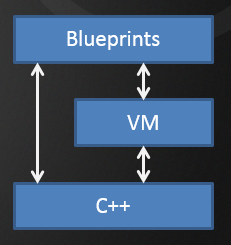
\includegraphics[scale=0.6]{blueVsC.png}
				\caption{结构图}
				\label{struct}
			\end{figure}
	
		
		\subsection{蓝图}
			\begin{itemize}
				\item 一种面向美术人员和设计师友好的可视化脚本系统
				\item 跟UnrealScript使用的相同的\textbf{虚拟机}
				\item 几乎跟UnrealScript一样强,在某些方面甚至更强
			\end{itemize}
		
		\subsection{C++}
			\begin{itemize}
				\item 一直是UE游戏编程中的一部分
				\item 跟虚拟机相互紧密地结合在一起
				\item 在UE4里面得到巨大的改进用来让编程人员替代UnrealScript
			\end{itemize}
		
		\subsection{蓝图 Vs C++}
			\begin{itemize}
				\item 蓝图适合快速迭代
				\item 蓝图比原生C++消耗更多的CPU性能
					\begin{itemize}
						\item 运行在虚拟机上
						\item 大约比原生C++代码慢8~10倍
						\item 对于大多数简单的事件驱动的任务,你可能并不会发现性能有什么大的消耗
						\item 许多发行的AAA游戏都在使用蓝图(包括Epic自己)
						\item 每帧需要更新的(tick)应用使用原生C++(物理模拟)
					\end{itemize}
				\item 但是,蓝图仍然很合适做原型开发
			\end{itemize}
			
			\paragraph{总结}
				\begin{itemize}
					\item 蓝图可以让设计师快速简单得实现想法
					\item 图状结构可以让程序员快速简单得用C++代码实现并优化
					\item 代码可以在编辑器中添加到任意工程中
					\item 快速协作、畅通沟通,不会出现模糊不清的玩法设计。
				\end{itemize}
				
				个人理解,蓝图系统非常强大,可用于快速原型设计、简单事件驱动玩法的开发,但是如果玩法复杂需要耗费非常多的CPU性能,那么最好把设计师使用蓝图设计的玩法翻译成原生的C++代码,如果本身一些像物理模拟等需要每帧更新又特别耗时的那么需要使用C++来进行开发。

	\section{参考}
			蛮牛课程:\url{http://edu.manew.com/course/101/reviews}
		
			\url{https://blog.csdn.net/kitok/article/details/80267273}
			
			蓝图入门:\url{https://www.cnblogs.com/ghl_carmack/p/5922131.html}
			
			UE4 笔记:\url{http://www.cnblogs.com/ghl_carmack/category/816351.html}
			
			

\chapter{蓝图类型}
	\section{关卡蓝图}

	\section{类蓝图}
	
	\section{仅包含数据的蓝图}
	
	\section{蓝图接口}
	
	\section{蓝图宏库}
	
	\section{参考} 
		UE4-2: \url{http://www.cnblogs.com/ghl_carmack/p/5922190.html}
	
	
\chapter{蓝图变量与流程控制}
	\section{变量类型}
		\subsection{变量概述}
		
		\subsection{基本类型}
		
		\subsection{蓝图数组}

	\section{流程控制}
		\subsection{概述}
		
		\subsection{开关节点}
		
		\subsection{Branch}
		
		\subsection{DoN}
		
		\subsection{DoOnce}
		
		\subsection{FlipFlop}
		
		\subsection{ForLoop}
		
		\subsection{ForLoopWithBreak}
		
		\subsection{Gate}
		
		\subsection{MultiGate}

		\subsection{Sequnce}
		
		\subsection{WhileLoop}
		
	\section{函数}
		\subsection{访问修饰符}
		
		\subsection{纯函数和非纯函数}
		
		\subsection{如何创建函数}
			\paragraph{在蓝图中创建}
			
			\paragraph{在蓝图接口中创建}
		
		\subsection{编辑函数}
		
		\subsection{调用函数}
	
	\section{参考}
		UE4-3: \url{http://www.cnblogs.com/ghl_carmack/p/5924965.html}


\chapter{蓝图与C++ 交互}
	

	\section{参考}
		UE4-4: \url{http://www.cnblogs.com/ghl_carmack/p/5925405.html}
		

\chapter{玻璃红外门} 


		    
\end{document} 
 		    